\documentclass[11pt]{article}
\usepackage{amsmath, amssymb, amsthm}
\usepackage{geometry}
\usepackage{hyperref}
\usepackage{booktabs}
\usepackage{xcolor}
\usepackage{listings}
\usepackage{tikz}

\geometry{margin=1.1in}

\newtheorem{lemma}{Lemma}
\newtheorem{fact}{Fact}
\newtheorem{remark}{Remark}

\newcommand{\eps}{\varepsilon}
\newcommand{\dt}{\Delta t}
\newcommand{\dx}{\Delta x}
\newcommand{\h}{h}
\newcommand{\code}[1]{\texttt{#1}}
\DeclareMathOperator*{\argmin}{arg\,min}

\lstset{
  basicstyle=\ttfamily\small,
  columns=fullflexible,
  keepspaces=true,
  breaklines=true,
  frame=single,
}

\title{Non-Uniform Time Grid, Take 2:\\ Defining the $x$- and $y$-Variable Grids}
\author{Optimal Transport / Schr\"odinger Bridge Project}
\date{}

\begin{document}
\maketitle

\begin{abstract}
This is a step-by-step, checkpointed re-derivation of the non-uniform (Chebyshev-clustered)
time grid used by the Python LADMM solver, written to be verified one section at a time
rather than accepted in one pass. \textbf{Step 1 (this section only): define the two grids
the splitting actually carries state on -- the $x$-variable (constraint) grid and the
$y$-variable (KE) grid -- and lay out where every field lives for the concrete case
$n_t=n_x=4$, space still uniform (1D).} No operators, no FP constraint, no projection yet --
those are later steps, once the grid itself is confirmed correct.
\end{abstract}

%------------------------------------------------------------------------------
\section{Naming: what ``$x$'' and ``$y$'' mean here}
\label{sec:naming}
%------------------------------------------------------------------------------

\textbf{This is a re-statement of an assumption, flagged for you to confirm or correct
before anything below is built on it.} The solver (\code{ladmm.py}) solves a
consensus-form problem
\[
  \min_{x,y} \; f_1(x) + f_2(y) \quad \text{s.t.} \quad A x + B y = d,
\]
where $x$ and $y$ are \emph{not} spatial coordinates -- they are the two copies of the
state that linearized ADMM carries:
\begin{itemize}
  \item $x = (q,b)$, code fields \code{rho\_stag}/\code{mx\_stag}: lives on the
        \textbf{constraint grid}, staggered, where the Fokker--Planck constraint is
        enforced \emph{exactly} (\code{projection\_nu.py}).
  \item $y = (\rho,m)$, code fields \code{rho\_cc}/\code{mx\_cc}: lives on the
        \textbf{KE grid}, collocated, where the kinetic-energy prox acts pointwise
        (\code{prox\_nu.py}).
\end{itemize}
As ambient (real) vector spaces -- shapes derived in \S\ref{sec:fields}, from the
staggered/collocated layouts of \code{operators.py}/\code{operators\_nu.py} --
\begin{equation}
  \label{eq:xy-spaces}
  x = (q,b) \in \mathbb{R}^{(n_t-1)n_x} \times \mathbb{R}^{n_t(n_x-1)},
  \qquad
  y = (\rho,m) \in \mathbb{R}^{n_t n_x} \times \mathbb{R}^{n_t n_x}.
\end{equation}
$d$ is the ADMM constant, \textbf{not} \code{ladmm.py}'s own \code{b} parameter (that
name is unavailable here regardless -- $b$ already names the $x$-variable's momentum
field) -- and, contrary to an earlier version of this note, \textbf{not} generally zero
either. \code{pipeline\_nu.py} does zero out its own \code{b}, but only because its
\code{A\_fn} is itself affine (bakes $\rho_0,\rho_1$ directly into the interpolation via
\code{interp\_t\_at\_phi}'s boundary arguments) rather than exposing that boundary part
separately; once $A$ is refactored to be genuinely linear (Step 5, \S\ref{sec:A-d}), the
leftover boundary contribution becomes exactly this $d$, generally nonzero. This matches
\code{nonuniform\_grid\_refine\_ends.tex} \S2's ``two grids.'' \emph{Space}
(the physical coordinate the density lives over) is a separate axis from either grid --
right now it is 1D and uniform; both grids share it. \textbf{If ``$x$ and $y$'' was meant
as two spatial dimensions instead, stop here and say so -- everything past this point
assumes the ADMM-splitting reading above.}

%------------------------------------------------------------------------------
\section{The time grid: Chebyshev--Gauss--Lobatto clustering}
\label{sec:time-grid}
%------------------------------------------------------------------------------

$n_t$ cells on $[0,1]$, edges $t_0=0<t_1<\cdots<t_{n_t}=1$. The reference (uniform)
partition is $\xi_j = j/n_t$, $j=0,\ldots,n_t$. The clustered edges are the
Chebyshev--Gauss--Lobatto map applied to $\xi$:
\begin{equation}
  \label{eq:cgl}
  t_j = \tfrac12\bigl(1-\cos(\pi\,\xi_j)\bigr), \qquad j = 0,\ldots,n_t.
\end{equation}
(Code: \code{clustered\_time\_grid(nt, strength=1.0)} in \code{time\_grid.py} -- taking
\code{strength=1} recovers exactly \eqref{eq:cgl}; \code{strength}$<1$ blends toward the
uniform $t_j=\xi_j$ and is a separate knob, not used below.) Widths and centers follow the
grid's own general construction (\code{\_time\_grid\_from\_edges}):
\[
  \dt_j = t_{j+1}-t_j \ (j=0,\ldots,n_t-1), \qquad \tau_j = \tfrac12(t_j+t_{j+1}).
\]
Clustering is quadratic at both ends: near $\xi=0$, $t\approx \tfrac{\pi^2}{4}\xi^2$, so
the first cell has width $O(1/n_t^2)$ instead of the uniform grid's $O(1/n_t)$; by
symmetry ($t_j = 1 - t_{n_t-j}$, since $\cos(\pi(1-\xi))=-\cos(\pi\xi)$) the same holds at
$\xi=1$. Mid-domain the map is close to linear, so cell widths there are close to
uniform.

%------------------------------------------------------------------------------
\section{The space grid: uniform (1D, for now)}
\label{sec:space-grid}
%------------------------------------------------------------------------------

Unchanged from \code{grid\_nu.py}/\code{grid.py}: $n_x$ cells on $[0,L]$ ($L=1$ below),
uniform width $\dx = L/n_x$, edges $x_k = k\,\dx$, cell centers $\xi_k =
(k-\tfrac12)\dx$.\footnote{Using $\xi_k$ for the space cell centers here follows
\code{nonuniform\_grid\_refine\_ends.tex}'s notation; unrelated to $\xi_j$ in
\S\ref{sec:time-grid}, which is the time reference partition. Sorry for the clash -- kept
for consistency with the earlier doc.} No clustering here yet -- this section is a
placeholder for whatever the analogous space construction turns out to be, once the time
grid above is confirmed.

%------------------------------------------------------------------------------
\section{Where each field lives}
\label{sec:fields}
%------------------------------------------------------------------------------

Combining \S\ref{sec:time-grid}--\ref{sec:space-grid} with the staggered/collocated
layouts from \code{operators.py}/\code{operators\_nu.py} (docstring: ``rho lives at
$(n_t{-}1,n_x)$ -- time-interior nodes, space cell-centers; mx lives at $(n_t,n_x{-}1)$ --
time cell-centers, space-interior nodes''):

\begin{center}
\begin{tabular}{lllcc}
\toprule
variable & field & locations & shape ($n_t,n_x$ general) & shape ($n_t{=}n_x{=}4$) \\
\midrule
$x=(q,b)$ & $q$ (density) & $(t_j,\xi_k)$, $j=1,\ldots,n_t{-}1$ & $(n_t{-}1)\times n_x$ & $3\times4=12$ \\
               & $b$ (momentum) & $(\tau_i,x_k)$, $k=1,\ldots,n_x{-}1$ & $n_t\times(n_x{-}1)$ & $4\times3=12$ \\
\midrule
$y=(\rho,m)$   & $\rho$ (density) & $(\tau_i,\xi_k)$, both centers & $n_t\times n_x$ & $4\times4=16$ \\
               & $m$ (momentum)   & $(\tau_i,\xi_k)$, both centers & $n_t\times n_x$ & $4\times4=16$ \\
\bottomrule
\end{tabular}
\end{center}

Flattening each field's 2D array of samples into a single real vector, in either order, is
exactly \S\ref{sec:naming}'s \eqref{eq:xy-spaces}: $q\in\mathbb{R}^{(n_t-1)n_x}$,
$b\in\mathbb{R}^{n_t(n_x-1)}$, $\rho,m\in\mathbb{R}^{n_t n_x}$.

Boundary data (fixed, not part of the unknowns): $q(t_0,\cdot)=\rho_0$,
$q(t_{n_t},\cdot)=\rho_1$ (the two marginals, sampled on the space grid of
\S\ref{sec:space-grid}); $b(\cdot,x_0)=b(\cdot,x_{n_x})=0$ (no-flux). Every $t_j$,
$\tau_i$ above is the \emph{clustered} value from \S\ref{sec:time-grid} -- this is the
only thing that changes relative to the uniform-time solver; every space location is
unchanged from \S\ref{sec:space-grid}.

%------------------------------------------------------------------------------
\section{Schematic: $n_t=n_x=4$}
\label{sec:schematic}
%------------------------------------------------------------------------------

Horizontal axis $x\in[0,1]$ (uniform); vertical axis $t\in[0,1]$ (clustered, drawn to
true scale -- the bunching near both ends is the actual geometry, not exaggerated). Left:
$x$-variable (constraint grid), staggered -- $q$ (circles) at time-edges $\times$
space-centers, $b$ (squares) at time-centers $\times$ space-edges, boundary data
(hollow) at the domain edges. Right: $y$-variable (KE grid), collocated -- $(\rho,m)$
(diamonds) at time-centers $\times$ space-centers only.

\begin{center}
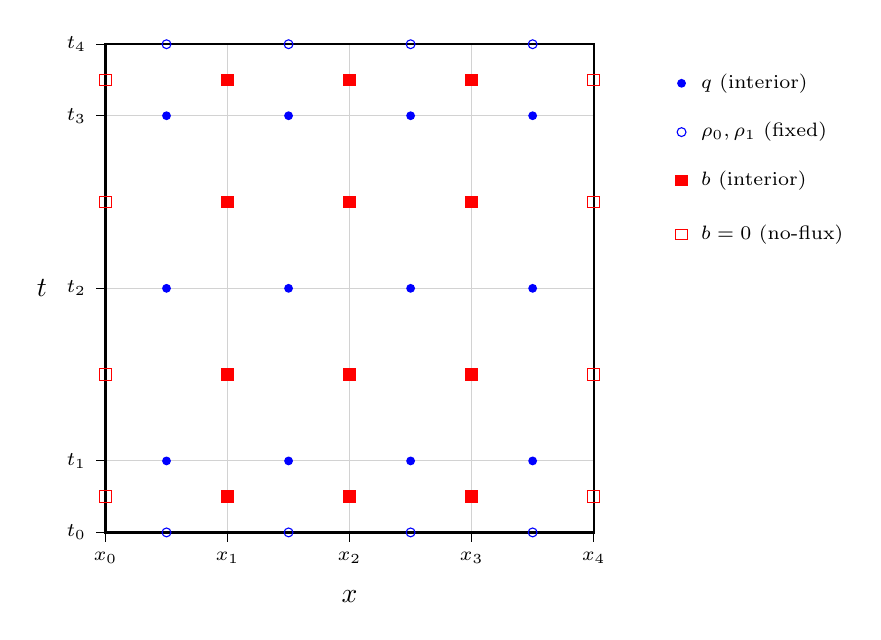
\begin{tikzpicture}[x=6.2cm, y=6.2cm]
  % ---- gridlines: space (uniform) ----
  \foreach \x in {0, 0.25, 0.5, 0.75, 1} {
    \draw[gray!35] (\x,0) -- (\x,1);
  }
  % ---- gridlines: time (clustered) ----
  \foreach \t in {0, 0.14645, 0.5, 0.85355, 1} {
    \draw[gray!35] (0,\t) -- (1,\t);
  }
  \draw[thick] (0,0) rectangle (1,1);

  % ---- axis ticks: space edges x_k ----
  \foreach \x/\lab in {0/{x_0}, 0.25/{x_1}, 0.5/{x_2}, 0.75/{x_3}, 1/{x_4}} {
    \draw (\x,0) -- (\x,-0.02) node[below, font=\scriptsize] {$\lab$};
  }
  % ---- axis ticks: time edges t_j ----
  \foreach \t/\lab in {0/{t_0}, 0.14645/{t_1}, 0.5/{t_2}, 0.85355/{t_3}, 1/{t_4}} {
    \draw (0,\t) -- (-0.02,\t) node[left, font=\scriptsize] {$\lab$};
  }
  \node[below] at (0.5,-0.1) {$x$};
  \node[left] at (-0.1,0.5) {$t$};

  % ---- x-variable: q (density) circles at (xi_k center, t_j interior) ----
  \foreach \t in {0.14645, 0.5, 0.85355} {
    \foreach \x in {0.125, 0.375, 0.625, 0.875} {
      \fill[blue] (\x,\t) circle (1.6pt);
    }
  }
  % ---- x-variable: b (momentum) squares at (x_k interior, tau_i center) ----
  \foreach \t in {0.07322, 0.32322, 0.67678, 0.92678} {
    \foreach \x in {0.25, 0.5, 0.75} {
      \draw[red, fill=red] (\x-0.012,\t-0.012) rectangle (\x+0.012,\t+0.012);
    }
  }
  % ---- boundary rho0/rho1: hollow circles at t=0, t=1 ----
  \foreach \x in {0.125, 0.375, 0.625, 0.875} {
    \draw[blue] (\x,0) circle (1.6pt);
    \draw[blue] (\x,1) circle (1.6pt);
  }
  % ---- no-flux b=0: hollow squares at x=0, x=1 ----
  \foreach \t in {0.07322, 0.32322, 0.67678, 0.92678} {
    \draw[red] (-0.012,\t-0.012) rectangle (0.012,\t+0.012);
    \draw[red] (0.988,\t-0.012) rectangle (1.012,\t+0.012);
  }

  % ---- legend ----
  \fill[blue] (1.18,0.92) circle (1.6pt); \node[right, font=\scriptsize] at (1.2,0.92) {$q$ (interior)};
  \draw[blue] (1.18,0.82) circle (1.6pt); \node[right, font=\scriptsize] at (1.2,0.82) {$\rho_0,\rho_1$ (fixed)};
  \draw[red, fill=red] (1.168,0.71) rectangle (1.192,0.73); \node[right, font=\scriptsize] at (1.2,0.72) {$b$ (interior)};
  \draw[red] (1.168,0.60) rectangle (1.192,0.62); \node[right, font=\scriptsize] at (1.2,0.61) {$b=0$ (no-flux)};
\end{tikzpicture}%
\hfill
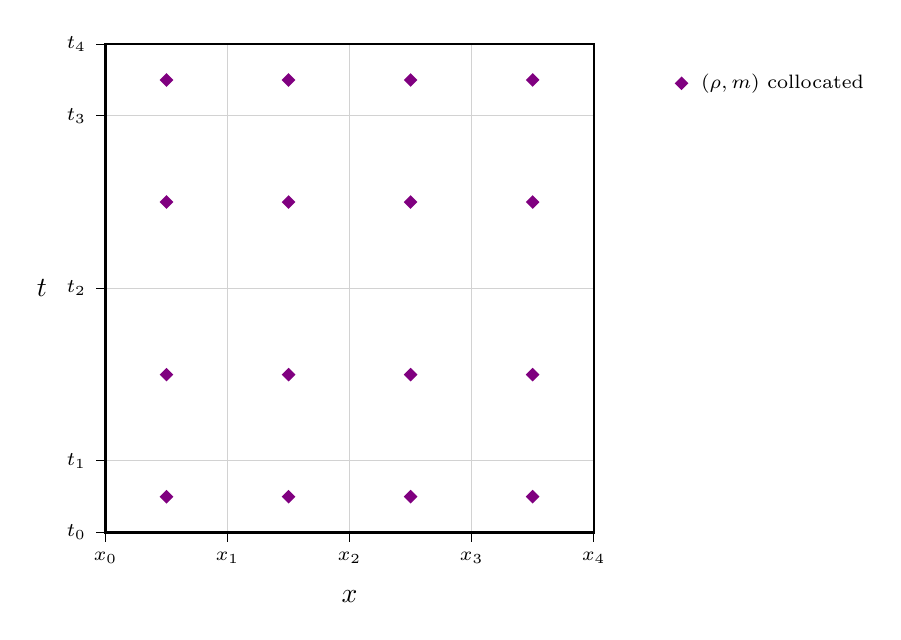
\begin{tikzpicture}[x=6.2cm, y=6.2cm]
  % ---- gridlines: space (uniform) ----
  \foreach \x in {0, 0.25, 0.5, 0.75, 1} {
    \draw[gray!35] (\x,0) -- (\x,1);
  }
  % ---- gridlines: time (clustered) ----
  \foreach \t in {0, 0.14645, 0.5, 0.85355, 1} {
    \draw[gray!35] (0,\t) -- (1,\t);
  }
  \draw[thick] (0,0) rectangle (1,1);

  \foreach \x/\lab in {0/{x_0}, 0.25/{x_1}, 0.5/{x_2}, 0.75/{x_3}, 1/{x_4}} {
    \draw (\x,0) -- (\x,-0.02) node[below, font=\scriptsize] {$\lab$};
  }
  \foreach \t/\lab in {0/{t_0}, 0.14645/{t_1}, 0.5/{t_2}, 0.85355/{t_3}, 1/{t_4}} {
    \draw (0,\t) -- (-0.02,\t) node[left, font=\scriptsize] {$\lab$};
  }
  \node[below] at (0.5,-0.1) {$x$};
  \node[left] at (-0.1,0.5) {$t$};

  % ---- y-variable: (rho,m) collocated diamonds at (xi_k, tau_i) ----
  \foreach \t in {0.07322, 0.32322, 0.67678, 0.92678} {
    \foreach \x in {0.125, 0.375, 0.625, 0.875} {
      \fill[violet] (\x,\t) ++(0,0.014) -- ++(0.014,-0.014) -- ++(-0.014,-0.014) -- ++(-0.014,0.014) -- cycle;
    }
  }
  \fill[violet] (1.18,0.92) ++(0,0.014) -- ++(0.014,-0.014) -- ++(-0.014,-0.014) -- ++(-0.014,0.014) -- cycle;
  \node[right, font=\scriptsize] at (1.2,0.92) {$(\rho,m)$ collocated};
\end{tikzpicture}
\end{center}

Note the visible clustering: the topmost/bottommost rows of $q$/$(\rho,m)$ points
(and the outer two rows of $b$-centers $\tau_0,\tau_3$) sit noticeably closer to
$t=0$/$t=1$ than the two middle rows, since \S\ref{sec:time-grid}'s $\dt_0=\dt_3
\approx 0.146 < \dt_1=\dt_2\approx 0.354$. Space spacing is uniform throughout (equal
column spacing in both panels).

%------------------------------------------------------------------------------
\section{Step 1: confirmed}
\label{sec:verify}
%------------------------------------------------------------------------------

\begin{enumerate}
  \item \textbf{Naming} (\S\ref{sec:naming}): $x=(q,b)$ on the constraint grid,
        $y=(\rho,m)$ on the KE grid. Confirmed.
  \item \textbf{Clustering}: full Chebyshev--Gauss--Lobatto (\S\ref{eq:cgl},
        \code{strength=1.0}), not the blended family. Confirmed.
  \item \textbf{Space}: uniform for this step (\S\ref{sec:space-grid} stays a
        placeholder); space-side clustering is out of scope until the time grid is
        settled. Confirmed.
  \item \textbf{Field placements} (\S\ref{sec:fields}, \S\ref{sec:schematic}): correct as
        drawn. Confirmed -- so whatever ``the wrong way'' referred to is \emph{not} the
        grid layout itself, and must be in something this step deliberately hasn't
        touched yet: the discrete FP constraint on the clustered grid, the projection
        that enforces it, or the KE prox's per-row weighting. Step 2 should pick one of
        those.
\end{enumerate}

%------------------------------------------------------------------------------
\section{Step 2: the kinetic-energy functional $f_2$}
\label{sec:f2}
%------------------------------------------------------------------------------

Discretize-first, optimize-second: write down the continuous objective, then discretize
it directly by quadrature on the $y$-grid already fixed in Step 1 -- no PDE, no
optimality conditions, no prox yet.

\subsection{The continuous functional}

The kinetic energy of a curve of measures $(\rho,m)$ on $[0,1]\times[0,L]$ is
\begin{equation}
  \label{eq:F2-continuous}
  \mathcal{F}_2[\rho,m] \;=\; \int_0^1\!\!\int_0^L L\bigl(\rho(t,x),\,m(t,x)\bigr)\,dx\,dt,
\end{equation}
where $L:\mathbb{R}\times\mathbb{R}\to(-\infty,+\infty]$ is the lower-semicontinuous
closure of $(\rho,m)\mapsto m^2/(2\rho)$:
\begin{equation}
  \label{eq:L}
  L(\rho,m) \;=\;
  \begin{cases}
    \dfrac{m^2}{2\rho}, & \rho > 0, \\[6pt]
    0, & \rho = 0,\ m = 0, \\[4pt]
    +\infty, & \text{otherwise (}\rho=0,\,m\neq0\text{ or }\rho<0\text{)}.
  \end{cases}
\end{equation}
$L$ is the perspective function of $\phi(u)=u^2/2$ (i.e.\ $L(\rho,m)=\rho\,\phi(m/\rho)$
for $\rho>0$), closed by taking its lsc envelope at $\rho=0$: since $\phi$ is convex with
superlinear growth, the only direction along which $L(\rho,m)$ stays finite as
$\rho\to0^+$ is $m\to0$ at the matching rate $m=O(\rho)$ (any fixed $m\neq0$ blows up like
$1/\rho$). This closure is what makes $L$ jointly convex and lsc on all of
$\mathbb{R}\times\mathbb{R}$ (not just $\{\rho>0\}$) -- the standard construction for the
Benamou--Brenier kinetic energy, needed here because the optimal $\rho$ can genuinely
vanish on part of the domain (e.g.\ Schr\"odinger-bridge solutions can be zero off the
support of $\rho_0,\rho_1$'s convex hull). $\code{prox\_ke\_cc}$'s \code{neg} clamp
(\code{rho\_new,mx\_new -> 0} whenever the cubic solve returns $\rho_{\mathrm{new}}\le
10^{-12}$) is exactly imposing this closure numerically: the only finite point on
$\{\rho=0\}$ is the origin, so the prox may only land \emph{there}, never at $\rho=0$
with $m\neq0$.

\subsection{Discretize: Riemann sum on the $y$-grid}

Step 1 fixed the $y$-grid at $(\tau_i,\xi_k)$, $i=0,\ldots,n_t-1$, $k=1,\ldots,n_x$, each
point the exact center of a cell of size $\Delta t_i\times\Delta x$ (midpoint rule, exact
for the cell-average of a linear function, same order of accuracy on the clustered grid as
on the uniform one -- $\Delta t_i$ varies by row but each cell's own midpoint is still
used for its own quadrature). The direct quadrature discretization of
\eqref{eq:F2-continuous} on this grid is
\begin{equation}
  \label{eq:f2-discrete}
  f_2(\rho,m) \;=\; \sum_{i=0}^{n_t-1}\sum_{k=1}^{n_x} \Delta t_i\,\Delta x\;
  L\bigl(\rho_{i,k},\,m_{i,k}\bigr), \qquad \rho_{i,k}:=\rho(\tau_i,\xi_k),\ \ m_{i,k}:=m(\tau_i,\xi_k),
\end{equation}
with $\Delta t_i$ the \emph{clustered} value from Step 1 \S\ref{sec:time-grid} and
$\Delta x=L/n_x$ constant (Step 1 \S\ref{sec:space-grid}). On the uniform-time grid
($\Delta t_i\equiv\Delta t=1/n_t$ for all $i$), \eqref{eq:f2-discrete} collapses to
$f_2 = \Delta t\,\Delta x\sum_{i,k}L(\rho_{i,k},m_{i,k})$ -- a single global constant times
an unweighted sum.

\subsection*{To verify before Step 3}

\begin{enumerate}
  \item Is \eqref{eq:F2-continuous}--\eqref{eq:L} the functional you meant -- kinetic
        energy only, no $\varepsilon$ (diffusion belongs to the FP constraint, i.e.\
        $f_1$/the projection, not here)?
  \item Is the discretize-first quadrature \eqref{eq:f2-discrete} -- midpoint rule, cell
        $\Delta t_i\times\Delta x$ centered at $(\tau_i,\xi_k)$ -- the intended
        discretization, or did you have a different quadrature in mind (e.g.\ one that
        doesn't use the cell \emph{center} as the sample point)?
\end{enumerate}

\textbf{Not doing yet:} reconciling \eqref{eq:f2-discrete} against \code{prox\_ke\_cc}/
\code{prox\_ke\_cc\_nu}'s actual code -- dropped per your flag that something about that
formulation is off. Once \S\ref{sec:f2} itself is settled, we can redo that comparison
from scratch rather than patch the previous version.

%------------------------------------------------------------------------------
\section{Step 3: the Fokker--Planck constraint}
\label{sec:fp}
%------------------------------------------------------------------------------

\subsection{Continuous constraint}

\begin{equation}
  \label{eq:fp-continuous}
  \partial_t \rho + \partial_x m \;=\; \varepsilon\,\partial_x^2\rho,
  \qquad (t,x)\in(0,1)\times(0,L),
\end{equation}
with $\rho(0,\cdot)=\rho_0$, $\rho(1,\cdot)=\rho_1$ (the two fixed marginals) and, at both
space boundaries, no advective \emph{and} no diffusive flux: $m(t,0)=m(t,L)=0$ and
$\partial_x\rho(t,0)=\partial_x\rho(t,L)=0$ (fully reflecting domain).

\subsection{Where it lands}

Discretize-first: $x=(q,b)$ carries the samples, but the residual is evaluated -- landed
-- on the \emph{same} grid as $y$ fixed in Step 1/2, $(\tau_i,\xi_k)$,
$i=0,\ldots,n_t{-}1$, $k=1,\ldots,n_x$. So the residual $R(q,b)$ is a field in
$\mathbb{R}^{n_t\times n_x}$ (flattened, $\mathbb{R}^{n_tn_x}$) -- the same ambient space
as \emph{each single field} of $y$ in \eqref{eq:xy-spaces}, not the same space as $x$
itself.

\subsection{The matrices}

Four building blocks, each acting along one axis only.

\textbf{Time derivative $\mathbf{D}_t$} (acts on each space column $q_{\cdot,k}\in
\mathbb{R}^{n_t-1}$ independently, using Step 1's clustered $\Delta t_i$):
\begin{equation}
  (D_t q)_{i,k} = \frac{q_{i+1,k}-q_{i,k}}{\Delta t_i}, \qquad q_{0,k}=\rho_0(\xi_k),\ \
  q_{n_t,k}=\rho_1(\xi_k),
\end{equation}
i.e.\ $D_t q = \mathbf{D}_t\,q_{\cdot,k} + r_t$, with $\mathbf{D}_t\in
\mathbb{R}^{n_t\times(n_t-1)}$ bidiagonal and $r_t$ the boundary contribution:
\begin{equation}
  \mathbf{D}_t =
  \begin{pmatrix}
    1/\Delta t_0 & & & \\
    -1/\Delta t_1 & 1/\Delta t_1 & & \\
     & \ddots & \ddots & \\
     & & -1/\Delta t_{n_t-2} & 1/\Delta t_{n_t-2} \\
     & & & -1/\Delta t_{n_t-1}
  \end{pmatrix}\!, \quad
  (r_t)_{i,k} =
  \begin{cases}
    -\rho_0(\xi_k)/\Delta t_0, & i=0, \\
    +\rho_1(\xi_k)/\Delta t_{n_t-1}, & i=n_t-1, \\
    0, & \text{else}.
  \end{cases}
\end{equation}

\textbf{Time average $\bar{\mathbf{I}}_t$} (same domain/BCs as $\mathbf D_t$, used only
inside the diffusion term -- this is exactly Lemma~1 of
\code{nonuniform\_grid\_refine\_ends.tex}, the exact midpoint interpolant):
\begin{equation}
  (\bar I_t q)_{i,k} = \tfrac12(q_{i,k}+q_{i+1,k}) = \bigl(\bar{\mathbf I}_t\,q_{\cdot,k}\bigr)_i + (s_t)_{i,k},
  \qquad
  \bar{\mathbf I}_t = \tfrac12\begin{pmatrix}
    1 & & & \\
    1 & 1 & & \\
     & \ddots & \ddots & \\
     & & 1 & 1 \\
     & & & 1
  \end{pmatrix}\!,
\end{equation}
$(s_t)_{i,k}=\rho_0(\xi_k)/2$ at $i=0$, $\rho_1(\xi_k)/2$ at $i=n_t{-}1$, else $0$.

\textbf{Space divergence $\mathbf{D}_x$} (acts on each time row $b_{i,\cdot}\in
\mathbb{R}^{n_x-1}$ independently; homogeneous -- no-flux $b_{i,0}=b_{i,n_x}=0$ needs no
affine term):
\begin{equation}
  (D_x b)_{i,k} = \frac{b_{i,k}-b_{i,k-1}}{\Delta x} = \bigl(\mathbf{D}_x\,b_{i,\cdot}\bigr)_k,
  \qquad
  \mathbf{D}_x = \frac{1}{\Delta x}\begin{pmatrix}
    1 & & & \\
    -1 & 1 & & \\
     & \ddots & \ddots & \\
     & & -1 & 1 \\
     & & & -1
  \end{pmatrix} \in \mathbb{R}^{n_x\times(n_x-1)}.
\end{equation}

\textbf{Space Laplacian $\mathbf{L}_x$} (acts on each time row of $\bar I_t q$
independently; homogeneous Neumann via ghost cells $g_0:=g_1$, $g_{n_x+1}:=g_{n_x}$, so
the two corner entries are $-1$ instead of $-2$):
\begin{equation}
  \bigl(L_x[g]\bigr)_{i,k} = \frac{g_{i,k+1}-2g_{i,k}+g_{i,k-1}}{\Delta x^2}
  = \bigl(\mathbf{L}_x\,g_{i,\cdot}\bigr)_k,
  \qquad
  \mathbf{L}_x = \frac{1}{\Delta x^2}
  \begin{pmatrix}
    -1 & 1 & & & \\
    1 & -2 & 1 & & \\
     & \ddots & \ddots & \ddots & \\
     & & 1 & -2 & 1 \\
     & & & 1 & -1
  \end{pmatrix} \in \mathbb{R}^{n_x\times n_x}.
\end{equation}

\subsection{Assembled}

\begin{equation}
  \label{eq:R}
  R(q,b) \;=\; D_t q \;+\; D_x b \;-\; \varepsilon\, L_x\bigl[\bar I_t q\bigr]
  \;\in\; \mathbb{R}^{n_t\times n_x},
\end{equation}
separable into a pure-time piece ($\mathbf D_t$, $\bar{\mathbf I}_t$, one independent
$(n_t{-}1)$- or $n_t$-vector problem per space column $k$) and a pure-space piece
($\mathbf D_x$, $\mathbf L_x$, one independent $(n_x{-}1)$- or $n_x$-vector problem per
time row $i$), never mixing the two within a single matrix.

$x=(q,b)$'s ambient space \eqref{eq:xy-spaces} only counts the \emph{free} (interior)
entries -- $\rho_0,\rho_1,0$ are fixed data, not unknowns -- so as a map on that space,
$R$ is affine, not linear, and the boundary contribution belongs explicitly on the
right-hand side, not folded silently into ``$D_tq$''/``$\bar I_tq$''. Writing $\mathbf
D_t,\bar{\mathbf I}_t$ acting on the free interior columns $q_{\cdot,k}$ alone (dropping
$r_t,s_t$ from \S\ref{sec:fp}.3):
\begin{equation}
  \label{eq:R-affine}
  R(q,b) \;=\; \mathbf D_t q \;+\; \mathbf D_x b \;-\; \varepsilon\,\mathbf L_x\bigl[\bar{\mathbf I}_t q\bigr]
  \;+\; r, \qquad r_{i,k} =
  \begin{cases}
    -\dfrac{\rho_0(\xi_k)}{\Delta t_0} \;-\; \varepsilon\bigl(\mathbf L_x[\rho_0/2]\bigr)_k, & i=0, \\[10pt]
    +\dfrac{\rho_1(\xi_k)}{\Delta t_{n_t-1}} \;-\; \varepsilon\bigl(\mathbf L_x[\rho_1/2]\bigr)_k, & i=n_t-1, \\[8pt]
    0, & \text{else.}
  \end{cases}
\end{equation}
Two contributions land in each of rows $i=0,n_t{-}1$: the direct $\pm\rho_\bullet/\Delta
t_\bullet$ term from $\mathbf D_t$'s own boundary rows ($r_t$), and, since $\bar{\mathbf
I}_t q$'s boundary rows feed straight into the \emph{linear} operator $\mathbf L_x$
(diffusion doesn't stop at the time boundary -- $\bar I_t q$ at $i=0$ is already
$\rho_0$-weighted, and $\mathbf L_x$ still acts on it in space), a second term
$-\varepsilon\,\mathbf L_x[s_t]$, i.e.\ the spatial Laplacian of the boundary
\emph{density profile itself} ($\rho_0(\cdot)/2$, not just its value at one point) --
this second piece is easy to drop (it vanishes only if $\rho_0,\rho_1$ happen to be
spatially constant) and is exactly the part missing from \eqref{eq:R}'s more compact
notation. $D_xb$ carries no such term: $b$'s boundary data is the homogeneous $0$, so
$\mathbf D_x b + 0 = D_x b$ already. The FP-feasible set is
\begin{equation}
  X = \{(q,b) : R(q,b) = 0\},
\end{equation}
and $f_1(x) = \iota_X(x)$ (the $\{0,+\infty\}$ indicator) -- so $\mathrm{prox}_{f_1}$ is
exactly the Euclidean projection onto $X$, i.e.\ \code{proj\_fokker\_planck\_banded\_nu}.
\emph{Solving} that projection (the $R R^{\!*}\phi = R(x)$ system) is a later step, not
here.

\subsection*{To verify before Step 4}

\begin{enumerate}
  \item Is \eqref{eq:fp-continuous} the constraint you meant, with both the advective
        \emph{and} diffusive flux vanishing at the space boundary?
  \item Landing location: $R(q,b)$ lives on the same $(\tau_i,\xi_k)$ grid as $y$, not on
        $x$'s own (staggered) grid -- correct?
  \item Do $\mathbf D_t,\bar{\mathbf I}_t,\mathbf D_x,\mathbf L_x$ in \S\ref{sec:fp}.3 match
        what you had in mind, in particular $\mathbf L_x$'s $-1$ (not $-2$) corner entries
        from the homogeneous-Neumann ghost?
  \item Does \eqref{eq:R-affine}'s boundary term $r$ now match what you had in mind --
        both the direct $\mathbf D_t$ piece \emph{and} the $-\varepsilon\,\mathbf
        L_x[\rho_0/2]$/$-\varepsilon\,\mathbf L_x[\rho_1/2]$ piece coming from the
        diffusion acting on the boundary-averaged density?
\end{enumerate}

%------------------------------------------------------------------------------
\section{Step 4: the linearized ADMM iteration (abstract)}
\label{sec:ladmm}
%------------------------------------------------------------------------------

Deliberately abstract: no formula for $A$, no choice of $\langle\cdot,\cdot\rangle_\mathcal{X},
\langle\cdot,\cdot\rangle_\mathcal{Y}$ yet. The point is to pin down the \emph{algorithm}
first, see exactly where $\mathcal X,\mathcal Y$ enter it, and only then (a later step)
choose them -- rather than assuming Euclidean, as \S\ref{sec:f2}'s dropped \S7.3 did,
before checking whether the algorithm actually needs that choice.

\subsection{Setup}

$x\in\mathcal X$ ($=(q,b)$-space, \eqref{eq:xy-spaces}), $y\in\mathcal Y$ ($=(\rho,m)$-space),
each equipped with an inner product ($\langle\cdot,\cdot\rangle_\mathcal{X},
\langle\cdot,\cdot\rangle_\mathcal{Y}$, hence norms $\|\cdot\|_\mathcal{X},
\|\cdot\|_\mathcal{Y}$) left \textbf{unspecified}. $f_1:\mathcal X\to(-\infty,+\infty]$ is
Step 3's FP-feasibility indicator $\iota_X$; $f_2:\mathcal Y\to(-\infty,+\infty]$ is
Step 2's kinetic energy \eqref{eq:f2-discrete}. $A:\mathcal X\to\mathcal Y$ and
$B:\mathcal Y\to\mathcal Y$ are the linear consensus maps of the constraint $Ax+By=d$
($d$, not \code{ladmm.py}'s \code{b}, to stay clear of $x=(q,b)$'s own $b$ -- \S\ref{sec:naming});
this problem's $B=-\mathrm{Id}_\mathcal{Y}$ is substituted directly below (every
$By\to -y$), while $d$ is left symbolic -- pinned down concretely in Step 5
(\S\ref{sec:A-d}). $A$ itself is not yet specified (``$A=I_t$'' was a placeholder name,
not a claim).

\subsection{The iteration}

This is Fang, He, Liu \& Yuan (2015)'s linearized-ADMM iteration -- the one
\code{ladmm.py} cites and implements -- written with $\gamma$ for their penalty parameter
$\rho$, $z^k$ for their dual iterate $\gamma^k$ (to free up $\gamma$; also $k$, not $t$,
for the iteration index, so it doesn't clash with the PDE time variable $t$ used
everywhere else in this note), the unlabeled norm as $\|\cdot\|_\mathcal{Y}$ and the
$G$-metric as $\|\cdot\|_\mathcal{Z}$ (a third, still-unspecified metric -- not assumed
equal to $\langle\cdot,\cdot\rangle_\mathcal{X}$, since $\|\cdot\|_\mathcal{Y}$'s argument
lives in $\mathcal Y$, $\|\cdot\|_\mathcal{Z}$'s in $\mathcal X$, but there is no reason
yet to expect the same metric governs both the $x$-update's proximal term and $\mathcal X$
itself), the transpose pairings as $\mathcal Y$-inner-products
($\mathbf x^T\mathbf A^T\gamma^k=\langle Ax,z^k\rangle_\mathcal{Y}$, similarly for $B$),
$B=-\mathrm{Id}_\mathcal{Y}$ substituted ($By\to -y$ throughout), and over-relaxation
fixed at $\alpha=1$ (dropping every $(1-\alpha)(\cdot)$ term):
\begin{align}
  x^{k+1} &= \argmin_{x\in\mathcal X}\Bigl\{\, f_1(x) - \langle Ax,z^k\rangle_\mathcal{Y}
    + \frac{\gamma}{2}\bigl\|Ax-y^k-d\bigr\|_\mathcal{Y}^2
    + \frac12\bigl\|x-x^k\bigr\|_\mathcal{Z}^2 \,\Bigr\}, \label{eq:ladmm-x}\\
  y^{k+1} &= \argmin_{y\in\mathcal Y}\Bigl\{\, f_2(y) + \langle y,z^k\rangle_\mathcal{Y}
    + \frac{\gamma}{2}\bigl\|Ax^{k+1}-y-d\bigr\|_\mathcal{Y}^2 \,\Bigr\}, \label{eq:ladmm-y}\\
  z^{k+1} &= z^k - \gamma\bigl(Ax^{k+1}-y^{k+1}-d\bigr). \label{eq:ladmm-z}
\end{align}
Everything above is well-posed as \emph{stated} regardless of $\langle\cdot,\cdot\rangle_
\mathcal{X},\langle\cdot,\cdot\rangle_\mathcal{Y},\langle\cdot,\cdot\rangle_\mathcal{Z}$ --
but which point each argmin actually picks out, and hence whether \eqref{eq:ladmm-x} is
\code{proj\_fokker\_planck\_banded\_nu} or \eqref{eq:ladmm-y} is \code{prox\_ke\_cc\_nu},
depends on that choice. None of the three is assumed here.

\subsection*{To verify}

\begin{enumerate}
  \item Do \eqref{eq:ladmm-x}--\eqref{eq:ladmm-z} match what you had in mind -- in
        particular the inner-product pairings $\langle Ax,z^k\rangle_\mathcal{Y},
        \langle y,z^k\rangle_\mathcal{Y}$ (rather than, say, $\langle x,A^*z^k\rangle_
        \mathcal{X}$, the equivalent $\mathcal X$-side pairing), and the sign flip on the
        $y$-update's linear term from substituting $B=-\mathrm{Id}_\mathcal{Y}$?
  \item $x,y,A,B,d$ as in \S\ref{sec:ladmm}.1 -- anything there you'd rather state
        differently before we go further?
  \item Next: pin down $A$ concretely, or
        $\langle\cdot,\cdot\rangle_\mathcal{X},\langle\cdot,\cdot\rangle_\mathcal{Y},
        \langle\cdot,\cdot\rangle_\mathcal{Z}$ directly?
\end{enumerate}

%------------------------------------------------------------------------------
\section{Step 5: $A$ and $d$, concretely}
\label{sec:A-d}
%------------------------------------------------------------------------------

\subsection{As coded}

\code{pipeline\_nu.py}'s consensus map:
\begin{lstlisting}[language=Python]
def A_fn(x):
    return State(
        rho=ops.interp_t_at_phi(x.rho, rho0, rho1),
        mx=ops.interp_x_at_phi(x.mx, zeros_nt, zeros_nt),
    )
\end{lstlisting}
time-average $q$ (boundary data $\rho_0,\rho_1$), space-average $b$ (boundary data $0$,
the same no-flux condition \S\ref{sec:fp}.3 already used) -- exactly ``the interpolation
operator in time and space (averaging)'' you described, and exactly \S\ref{sec:fp}.3's
$\bar I_t$ applied to $q$, plus a new space twin applied to $b$.

\subsection{Splitting off the boundary part}

$\bar I_t q$ already has its affine part identified (\S\ref{sec:fp}.3): $\bar I_t q =
\bar{\mathbf I}_t q + s_t$. The space average of $b$ needs its own building block,
$\bar{\mathbf I}_x$ -- same construction as $\mathbf D_x$ (\S\ref{sec:fp}.3: same domain
$b_{i,\cdot}\in\mathbb R^{n_x-1}$, same $b_{i,0}=b_{i,n_x}=0$ boundary), averaging instead
of differencing:
\begin{equation}
  (\bar I_x b)_{i,k} = \tfrac12(b_{i,k-1}+b_{i,k}) = \bigl(\bar{\mathbf I}_x\,b_{i,\cdot}\bigr)_k,
  \qquad
  \bar{\mathbf I}_x = \tfrac12\begin{pmatrix}
    1 & & & \\
    1 & 1 & & \\
     & \ddots & \ddots & \\
     & & 1 & 1 \\
     & & & 1
  \end{pmatrix} \in \mathbb{R}^{n_x\times(n_x-1)},
\end{equation}
with \textbf{no} affine term: the boundary value being averaged in is $0$, the same
reason $\mathbf D_x$ needed none.

Writing $A(q,b):=(\bar{\mathbf I}_t q,\ \bar{\mathbf I}_x b)$ for the purely linear part
(acting on the free/interior $(q,b)$ only):
\begin{equation}
  \label{eq:A-full}
  A_{\mathrm{full}}(q,b) \;=\; A(q,b) \;+\; (s_t,\,0).
\end{equation}

\subsection{The constant $d$}

The original (code-level) constraint is $A_{\mathrm{full}}(x)-y=0$ ($B=-\mathrm{Id}_
\mathcal{Y}$, code's \code{b}$=0$, \S\ref{sec:naming}). Substituting \eqref{eq:A-full}:
\[
  A(x) + (s_t,0) - y = 0 \quad\Longleftrightarrow\quad A(x) - y = -(s_t,0),
\]
i.e., matching $Ax+By=d$ ($B=-\mathrm{Id}_\mathcal{Y}$):
\begin{equation}
  \label{eq:d}
  d = -(s_t,\,0) \in \mathcal Y, \qquad
  (d_\rho)_{i,k} =
  \begin{cases}
    -\rho_0(\xi_k)/2, & i=0,\\
    -\rho_1(\xi_k)/2, & i=n_t-1,\\
    0, & \text{else},
  \end{cases}
  \qquad d_m = 0.
\end{equation}
$d$ lives only in the density slot of $\mathcal Y$, only in its two boundary time-rows,
and is exactly minus the same boundary average $s_t$ already computed for the FP residual
in \S\ref{sec:fp}.3 -- no new boundary data, just the other place it enters.

\subsection*{Step 5: confirmed}

\begin{enumerate}
  \item $A(q,b)=(\bar{\mathbf I}_t q,\bar{\mathbf I}_x b)$ -- \eqref{eq:A-full} minus its
        affine part. Confirmed.
  \item \eqref{eq:d}'s $d$, including the momentum slot $d_m=0$. Confirmed.
\end{enumerate}

With $A$ and $d$ pinned down, the open question is now exactly what \S\ref{sec:ladmm}
deferred: what $\langle\cdot,\cdot\rangle_\mathcal{X},\langle\cdot,\cdot\rangle_\mathcal{Y},
\langle\cdot,\cdot\rangle_\mathcal{Z}$ should be. Per \S\ref{sec:ladmm}--\S\ref{sec:A-d},
each is (has to be, for the algorithm in \S\ref{sec:ladmm} to be well-posed at all) an SPD
matrix norm $\|v\|_M=\sqrt{v^TMv}$; the next step is choosing $M_\mathcal{X},M_\mathcal{Y},
M_\mathcal{Z}$.

%------------------------------------------------------------------------------
\section{Step 6: Pinning down $\mathcal X,\mathcal Y,\mathcal Z$}
\label{sec:norms-pinned}
%------------------------------------------------------------------------------

\subsection{$\mathcal X$ and $\mathcal Y$}

$\langle\cdot,\cdot\rangle_\mathcal X:=\langle\cdot,\cdot\rangle_N$,
$\langle\cdot,\cdot\rangle_\mathcal Y:=\langle\cdot,\cdot\rangle_M$, where $N,M$ are the
quadrature-consistent diagonal matrices of \code{nonuniform\_grid\_norms.tex} \S1 --
already \code{pipeline\_nu.py}'s \code{norm\_fn}/\code{dual\_norm\_fn}, promoted here
from diagnostic to the actual ADMM metric. That companion note also derives $A$'s
$N,M$-weighted adjoint $A^*=N^{-1}A^TM$ (equivalently $NA^*=A^TM$, used repeatedly below)
in closed form, and proves $\|A^*A\|_N=\|A\|_{\mathcal X\to\mathcal Y}^2\le1$ -- both facts
this section builds on directly.

\subsection{$\mathcal Z$}

Define $G:=\tau I-\gamma A^*A$ (an operator $\mathcal X\to\mathcal X$; $A^*A$ as a plain
matrix is $N^{-1}A^TMA$, so $G=\tau I-\gamma N^{-1}A^TMA$). Take
\begin{equation}
  \label{eq:MZ}
  \langle\cdot,\cdot\rangle_\mathcal Z := \langle\cdot,\cdot\rangle_{NG}, \qquad
  \|v\|_\mathcal Z^2 := v^T(NG)v,
\end{equation}
i.e.\ $M_\mathcal Z=NG$.

\begin{remark}
\textbf{Order matters here: $NG\ne GN$ in general, and only $NG$ is symmetric.} $(NG)^T=
G^TN=(\tau I-\gamma A^TMAN^{-1})N=\tau N-\gamma A^TMA=NG$ (using $NA^*=A^TM\Rightarrow
A^TMAN^{-1}=(NA^*A)N^{-1}$, so $G^T=\tau I-\gamma A^TMAN^{-1}$) -- so $NG$ is genuinely
symmetric, hence a valid candidate for an SPD matrix norm. $GN$, by the same computation
with the factors swapped, is symmetric only if $N$ and $A^*A$ commute, which they have no
reason to here. So $\|\cdot\|_\mathcal Z$ must be built from $NG$, not $GN$.
\end{remark}

\subsection{Collapsing the $x$-update to a projection under $N$}
\label{sec:collapse}

Substituting $\mathcal X=N,\mathcal Y=M,\mathcal Z=NG$ into \eqref{eq:ladmm-x}, expand
using $\langle Ax,z^k\rangle_M=\langle x,A^*z^k\rangle_N$ and $e^k:=y^k+d$:
\[
  -\langle Ax,z^k\rangle_M+\frac\gamma2\|Ax-e^k\|_M^2
  = \frac\gamma2\langle x,A^*Ax\rangle_N - \langle x,A^*(z^k+\gamma e^k)\rangle_N
  + \text{const}.
\]
Writing every term as a plain array pairing ($\langle x,w\rangle_N=x^TNw$, so
$\langle x,A^*Ax\rangle_N=x^T(NA^*A)x=x^T(A^TMA)x$) and adding $\tfrac12\|x-x^k\|_\mathcal
Z^2=\tfrac12x^T(NG)x-x^T(NG)x^k+\text{const}$, the full $x$-dependent part of
\eqref{eq:ladmm-x} is
\[
  x^T\Bigl[\tfrac\gamma2A^TMA+\tfrac12NG\Bigr]x
  \;-\; x^T\Bigl[NA^*(z^k+\gamma e^k)+NGx^k\Bigr] \;+\; \text{const}.
\]
\textbf{Quadratic term:} $\tfrac\gamma2A^TMA+\tfrac12NG=\tfrac\gamma2NA^*A+\tfrac12N(\tau
I-\gamma A^*A)=\tfrac\tau2N$ -- the $A^*A$ pieces cancel \emph{exactly}, which is the whole
point of \eqref{eq:MZ}'s choice of $G$: it is \emph{forced}, not guessed, by requiring
this cancellation.
\textbf{Linear term:} matching $x^T[\ldots]$ against $\tau x^TNw^k$ (the linear term of
$\tfrac\tau2\|x-w^k\|_N^2$) and dividing by $N$ (invertible):
\[
  \tau w^k = A^*(z^k+\gamma e^k) + Gx^k
  = A^*(z^k+\gamma e^k) + \tau x^k - \gamma A^*Ax^k
  = \tau x^k + A^*\bigl[z^k+\gamma(e^k-Ax^k)\bigr].
\]
Defining $r^k:=Ax^k-y^k-d$ (the constraint violation at the \emph{current}, not yet
updated, iterate -- note the $-d$: with $d$ generally nonzero (\S\ref{sec:A-d}), this
corrects the earlier abstract iteration's implicit $d=0$ assumption) so that
$e^k-Ax^k=-r^k$, and $g^k:=A^*(\gamma r^k-z^k)$:
\begin{equation}
  \label{eq:collapse}
  w^k = x^k - \tfrac1\tau g^k, \qquad
  x^{k+1} = \argmin_{x\in\mathcal X}\Bigl\{f_1(x) + \tfrac\tau2\|x-w^k\|_N^2\Bigr\}.
\end{equation}
This is exactly a projection (w.r.t.\ $N$) of the point $x^k-g^k/\tau$ onto the
FP-feasible set $X=\{R=0\}$ (\S\ref{sec:fp}.4) -- the same ``linearized gradient step,
then prox'' shape the abstract iteration always had in spirit, now derived (not assumed)
from the concrete choice of $\mathcal Z$. Two separate pieces of machinery are involved,
and only one is done: computing $g^k$ needs $A$'s weighted adjoint $A^*$, already in hand
(\code{nonuniform\_grid\_norms.tex} \S4--\S5); \emph{solving} \eqref{eq:collapse}'s
projection needs $R$'s own weighted adjoint (\code{projection\_nu.py}'s
\code{\_probe\_composite\_ops}/\code{thomas\_batch\_solve\_general} machinery, currently
assembled by probing $R$'s \emph{Euclidean} transpose) -- built the same way $A_t^*$ was,
but for $R$'s different combination of $\mathbf D_t,\bar{\mathbf I}_t,\mathbf D_x,\mathbf
L_x$ (\S\ref{sec:fp}.3), plus a still-unassigned metric on the residual/dual-potential
$\phi$ space. Not yet derived.

\subsection{$G\succeq0$ is automatic}

\eqref{eq:MZ} is only a valid metric if $M_\mathcal Z=NG$ is SPD, i.e.\ $G\succeq0$, i.e.\
$\tau I\succeq\gamma A^*A$, i.e.\ $\tau\ge\gamma\|A\|_{\mathcal X\to\mathcal Y}^2$ (the
generalized-Rayleigh-quotient characterization of the operator norm). This is exactly
\code{nonuniform\_grid\_norms.tex} \S7's stability condition -- already proved to hold
for $\tau>\gamma$, unconditionally, on any grid in this family. So $\mathcal Z$ is
guaranteed well-defined by a bound already established, not a new condition to check.

\subsection{The iteration, purely in terms of $N$ and $M$}
\label{sec:final-iteration}

Collecting: \eqref{eq:ladmm-x}--\eqref{eq:ladmm-z} with every $\mathcal X,\mathcal Y,
\mathcal Z$ replaced by $N,M,NG$ and simplified as far as it goes.

\textbf{$x$-update} -- already done, \eqref{eq:collapse}:
\begin{equation}
  \label{eq:final-x}
  x^{k+1} = \argmin_{x\in\mathcal X}\Bigl\{f_1(x)+\tfrac\tau2\|x-w^k\|_N^2\Bigr\},
  \qquad w^k = x^k-\tfrac1\tau A^*(\gamma r^k-z^k),
  \qquad r^k=Ax^k-y^k-d.
\end{equation}
No further simplification is available here -- $f_1=\iota_X$ isn't itself a sum of
independent per-point pieces (\S\ref{sec:fp}: $R$ couples neighboring $t_j$'s and
$x_k$'s), so \eqref{eq:final-x} is already in its simplest form; \emph{solving} it is
\S\ref{sec:collapse}'s open item, not a simplification of the argmin's statement.

\textbf{$y$-update} -- same completing-the-square move as \eqref{eq:collapse}, applied to
\eqref{eq:ladmm-y} with $\mathcal Y=M$ ($v^k:=(Ax^{k+1}-d)-z^k/\gamma$):
\[
  y^{k+1} = \argmin_{y\in\mathcal Y}\Bigl\{f_2(y)+\tfrac\gamma2\|y-v^k\|_M^2\Bigr\}.
\]
Unlike $f_1$, $f_2$ \emph{is} a sum of independent per-point terms
(\eqref{eq:f2-discrete}: $f_2(y)=\sum_{i,k}\dt_i\dx\,L(\rho_{i,k},m_{i,k})$), and $M$
carries \emph{the same} per-point weight $\dt_i\dx$ by construction (\S\ref{sec:norms-pinned}.1)
-- so $\|y-v^k\|_M^2=\sum_{i,k}\dt_i\dx\big[(\rho_{i,k}-v^k_{\rho,i,k})^2+(m_{i,k}-v^k_
{m,i,k})^2\big]$ shares the identical weight, term by term, with $f_2$. The full objective
is then $\sum_{i,k}\dt_i\dx\big[L(\cdot,\cdot)+\tfrac\gamma2(\cdot,\cdot)\big]$, a sum of
independent terms each scaled by a positive constant that cannot move that term's own
minimizer -- so the $\dt_i\dx$ cancels entirely, point by point:
\begin{equation}
  \label{eq:final-y}
  (\rho^{k+1}_{i,k},m^{k+1}_{i,k}) = \argmin_{\rho,m}\Bigl\{L(\rho,m)+\tfrac\gamma2\bigl[
  (\rho-v^k_{\rho,i,k})^2+(m-v^k_{m,i,k})^2\bigr]\Bigr\}, \qquad \forall (i,k).
\end{equation}
No $\dt_i$, no $\dx$, anywhere -- \eqref{eq:final-y} is \emph{exactly}
\code{prox\_ke\_cc}'s uniform-grid cubic solve, at the constant step $\sigma=1/\gamma$,
called pointwise. This is the simplest the $y$-update can possibly get: strictly simpler
than \code{prox\_ke\_cc\_nu}'s current per-row $\sigma_{\mathrm{eff}}=\sigma\,\dt_i/\dt_
{\mathrm{ref}}$ rescaling, which becomes not just unnecessary but wrong to keep once $M$
is the genuine metric (it was compensating for a mismatch -- weighted $f_2$, unweighted
penalty -- that \eqref{eq:final-y} shows doesn't exist here).

\textbf{$z$-update} -- \eqref{eq:ladmm-z} is a plain vector formula, never inside a norm
or inner product on either side; substituting $\mathcal Y=M$ changes nothing about it:
\begin{equation}
  \label{eq:final-z}
  z^{k+1} = z^k-\gamma\bigl(Ax^{k+1}-y^{k+1}-d\bigr).
\end{equation}
($z^k$ lives in $(\mathcal Y,M)$ -- its \emph{norm}, if ever reported as a diagnostic,
would use $M$ -- but the update rule itself is metric-independent, so there is nothing
left to simplify.)

\subsection*{To verify}

\begin{enumerate}
  \item $\mathcal X=N,\mathcal Y=M$ (\S\ref{sec:norms-pinned}.1) -- the intended pinning?
  \item $\mathcal Z=NG$, not $GN$ (\S\ref{sec:norms-pinned}.2's Remark) -- does the
        asymmetry argument hold up, or was $GN$ actually intended in some other sense
        (e.g.\ as a right-acting operator, not a symmetric bilinear form)?
  \item \eqref{eq:collapse}'s derivation -- every step, in particular the corrected
        $r^k:=Ax^k-y^k-d$ (now including $-d$) -- any gap?
  \item \S\ref{sec:final-iteration}'s three final forms -- \eqref{eq:final-x}
        (unchanged/unsimplifiable), \eqref{eq:final-y} (the $\dt_i\dx$ cancellation,
        landing exactly on \code{prox\_ke\_cc}), \eqref{eq:final-z} (no simplification
        applies) -- correct, and is \eqref{eq:final-y}'s claim that
        \code{prox\_ke\_cc\_nu}'s $\sigma_{\mathrm{eff}}$ rescaling should go away
        entirely (not just simplify) the conclusion you expected?
  \item Next: derive $R$'s $N$-weighted adjoint (redoing \S\ref{sec:fp}'s projection under
        $N$), which is what \eqref{eq:final-x} still needs before it's fully concrete?
\end{enumerate}
\end{document}
